\documentclass{article}

\usepackage{geometry}
\geometry{left=1.5in,right=1.5in,top=1.25in,bottom=1.25in}

\usepackage{listings}
\usepackage{color}
\usepackage{xcolor}
\usepackage{longtable}
\usepackage{amssymb}
\usepackage{array}
\usepackage[bahasa]{babel}
\usepackage{courier}
\usepackage{graphicx}
\usepackage{tikz} 
\usepackage{tikz,pgfplots}
\usepackage{amsmath}

\definecolor{codegreen}{rgb}{0,0.6,0}
\definecolor{codeblue}{rgb}{0,0,0.6}
\definecolor{codegray}{rgb}{0.5,0.5,0.5}
\definecolor{codepurple}{rgb}{0.58,0,0.82}
\definecolor{backcolour}{rgb}{0.95,0.95,0.92}

\lstdefinestyle{mystyle}{
    backgroundcolor=\color{backcolour},   
    commentstyle=\color{codegray},
    keywordstyle=\color{codepurple}\bfseries,
    numberstyle=\tiny\color{codegray}\ttfamily,
    stringstyle=\color{codegreen},
    identifierstyle=\color{codeblue},
    basicstyle=\scriptsize\ttfamily,
	xleftmargin=2em,frame=single,framexleftmargin=1.5em,  
	rulecolor=\color{codegray},
    breaklines=true,                  
    keepspaces=true,               
    captionpos=b,                  
    numbers=left,                    
    numbersep=5pt,                  
    showspaces=false,                
    showstringspaces=false,
    showtabs=false,                  
    tabsize=2
}
 
\lstset{style=mystyle}

\title{Tugas Kecil Pengurutan Data dengan Algoritma \textit{Divide and Conquer}}
\author{Dery Rahman A, 13515097, K-01}
\date{Senin, 27 Februari 2017}

\begin{document}

	\pagenumbering{gobble}
	\maketitle

	\newpage
	\pagenumbering{arabic}

	\section{Deskripsi Permasalahan}
	\par Tugas kecil ini adalah mengimplementasikan 4 algoritma sorting \textit{Divide and Conquer} (yaitu \textit{MergeSort}, \textit{InsertionSort}, \textit{SelectionSort}, dan \textit{QuickSort}), lalu mengujinya dengan data yang besar. Input berupa koleksi data yang di\textit{generate} secara random mulai dari \textit{data set} berukuran 1000, 5.000, 10.000, 50.000, 100.000, 500.000, hingga 1.000.000. Koleksi data random didapatkan dengan menggunakan fungsi atau kelas Random. 
	\par Untuk mengukur kecepatan algoritma, gunakan method untuk mendapatkan waktu (\textit{current Time}) sebelum dan sesudah algoritma pengurutan dieksekusi, lalu hitung selisih antara kedua waktu. Proses \textit{generate} koleksi data secara random tidak perlu diukur kecepatannya. Sebelum mengukur kecepatan eksekusi algoritma, lakukan dulu pengecekan kebenaran hasil pengurutan yang diberikan oleh setiap algoritma.
	\par Lakukanlah perbandingan kecepatan eksekusi untuk keempat algoritma tersebut dengan menampilkannya dalam bentuk tabel dan chart. Berikanlah analisis sesuai dengan konsep yang dipelajari di kelas.

	\section{Algoritma \textit{Divide and Conquer}}
	\par \textit{Divide and Conquer} merupakan metode pemecahan masalah dengan cara membagi \textit{problem} menjadi \textit{subproblem} yang lebih kecil. Kemudian \textit{subproblem} tersebut diselesaikan secara independen dan selanjutnya menggabungkan solusi dari masing-masing \textit{subproblem} tersebut menjadi solusi \textit{problem} semula. Secara umum, algoritma \textit{Divide and Conquer} dibagi menjadi 3 proses :
	\begin{enumerate}
		\item \textit{Divide} : Membagi \textit{problem} menjadi beberapa \textit{subproblem} yang memiliki ukuran yang lebih kecil dari \textit{problem} semula, untuk kemudian dapat diselesaikan secara independen.
		\item \textit{Conquer} : Memecahkan masing-masing \textit{subproblem} tersebut (secara rekursif).
		\item \textit{Combine} : Menggabungkan solusi dari \textit{subproblem} tersebut menjadi solusi \textit{problem} semula.
	\end{enumerate}
	\par Dalam metode pengurutan menggunakan \textit{Divide and Conquer}, dapat dilakukan dengan 2 pendekatan :
	\begin{enumerate}
		\item Mudah membagi, sulit menggunakan : urut-gabung \textit{Merge sort} dan urut-sisip \textit{Insertion sort}
		\item Sulit membagi, mudah menggunakan : urut-cepat \textit{Quick sort} dan urut-seleksi \textit{Selection sort}
	\end{enumerate}
	
	\clearpage
	\section{\textit{Source} Program}

	\lstinputlisting[language=C++,caption=Implementasi \textit{Merge Sort}]{MergeSort.cpp}
	\lstinputlisting[language=C++,caption=Implementasi \textit{Insertion Sort}]{InsertionSort.cpp}
	\lstinputlisting[language=C++,caption=Implementasi \textit{Quick Sort}]{QuickSort.cpp}
	\lstinputlisting[language=C++,caption=Implementasi \textit{Selection Sort}]{SelectionSort.cpp}
	\lstinputlisting[language=C++,caption=Implementasi generate program random]{RandomGenerator.cpp}
	\lstinputlisting[language=C++,caption=Implementasi file \textit{Bash} generate program random]{rand.sh}
	\lstinputlisting[language=C++,caption=Implementasi file \textit{Bash} generate seluruh algoritma]{compile_run.bash}
	\lstinputlisting[language=C++,caption=Program cek kebenaran terurut]{CekSort.cpp}
	\lstinputlisting[language=C++,caption=Implementasi file \textit{Bash} cek terurut]{cek_sort.sh}
	\section{Contoh \textit{Input} dan \textit{Output}}
	\begin{table}[h]
		\small
		\newcolumntype{L}{>{\arraybackslash}m{.4\linewidth}}
		\centering		
		\begin{tabular}{|L|L|}
			\hline
			\textit{Input} & \textit{Output} \\
			\hline
			10 & \\
			4 7 0 0 2 3 0 5 6 0 & 0 0 0 0 2 3 4 5 6 7 \\
			\hline
			15 & \\
			10 2 90 1 1 -1 0 2 0 9 10 9 2 -10 -1 & -10 -1 -1 0 0 1 1 2 2 2 9 9 10 10 90 \\
			\hline
			10 & \\
			90 87 65 43 33 22 12 8 6 1 & 1 6 8 12 22 33 43 65 87 90 \\
			\hline
			15 & \\
			90 87 65 43 33 22 12 8 6 1 0 -1 -5 -8 -10 & -10 -8 -5 -1 0 1 6 8 12 22 33 43 65 87 90 \\
			\hline
		\end{tabular}
		\caption{Contoh \textit{input} dan \textit{output}}
	\end{table}
	
	\begin{figure}[h]
	\vspace*{-0.2in}
		\centerline{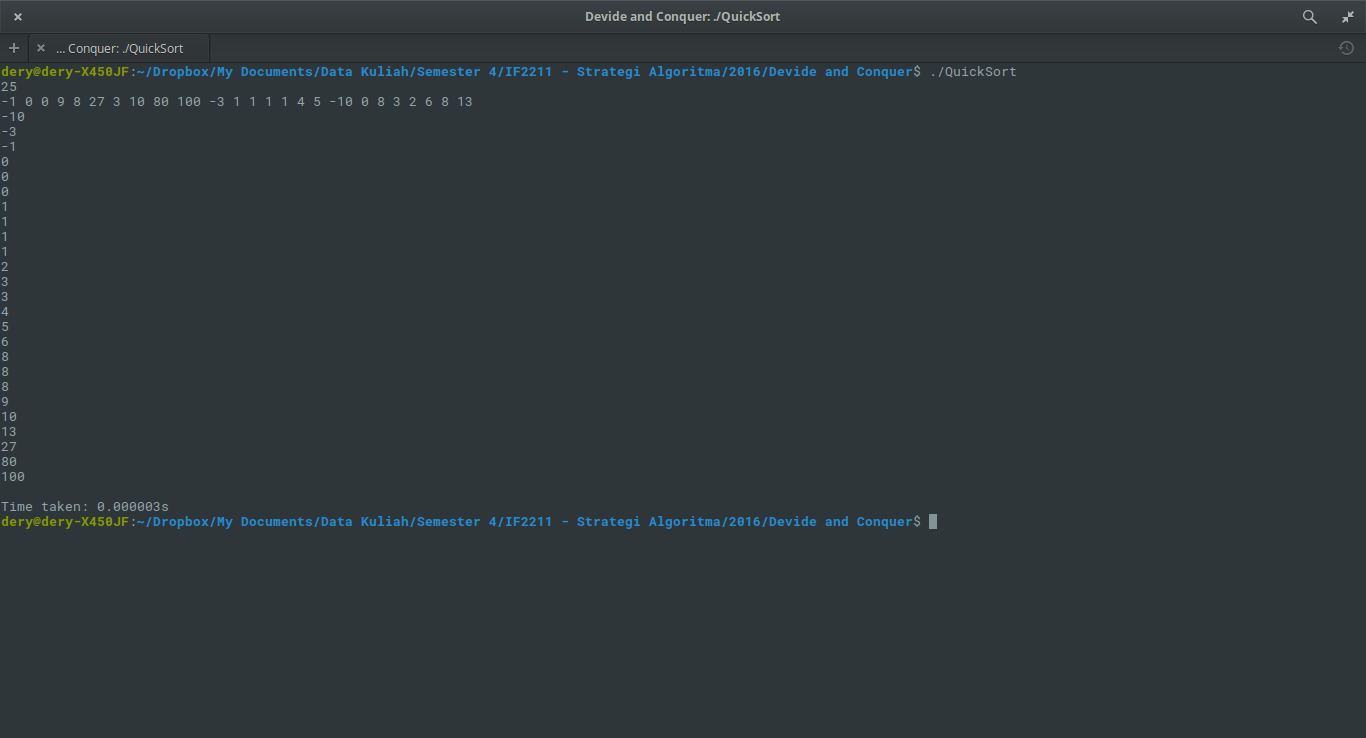
\includegraphics[width=\linewidth]{images/input-output.png}}
		\caption{Contoh \textit{input} dan \textit{output}}
	\end{figure}
	\clearpage
	\begin{figure}[h]
	\vspace*{-0.2in}
		\centerline{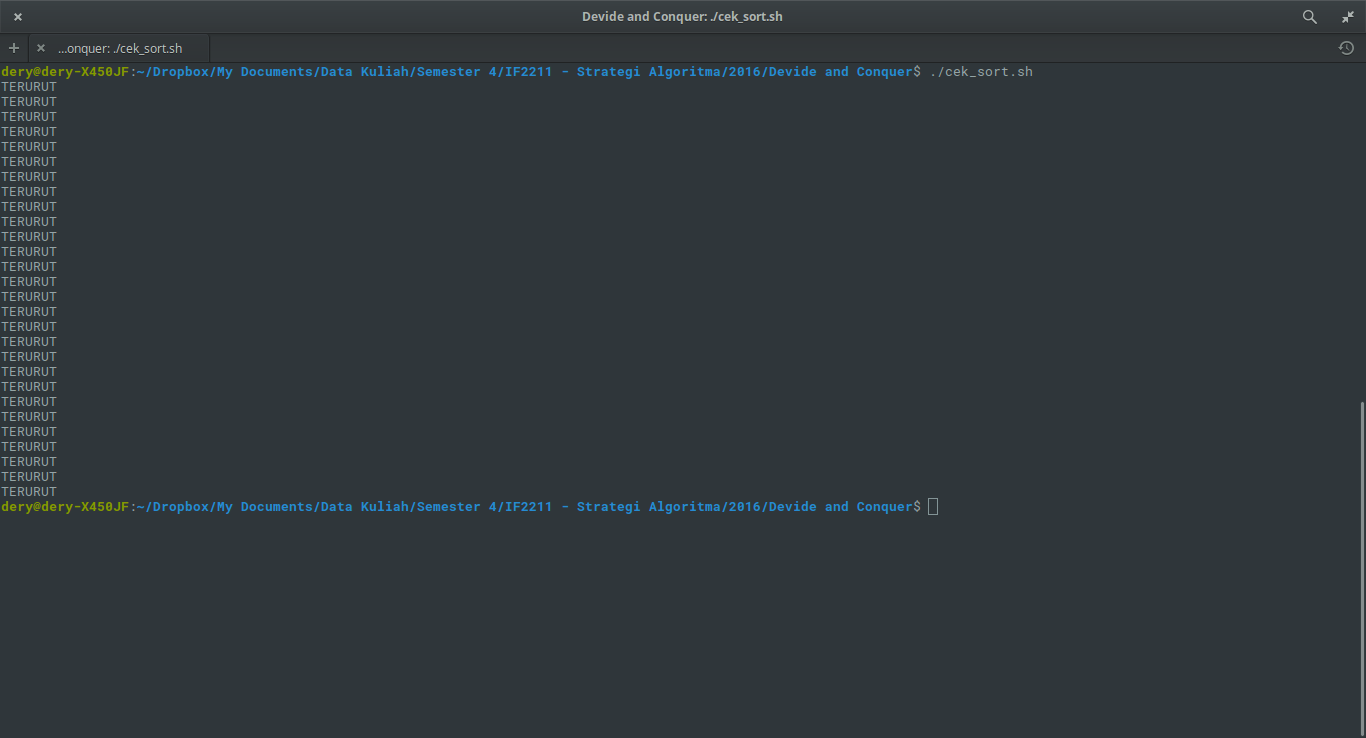
\includegraphics[width=\linewidth]{images/cek.png}}
		\caption{Cek keterurutan}
	\end{figure}

	\clearpage
	\section{Hasil Perbandingan dan Analisis}
	\par \textit{Data set} yang digunakan merupakan sekumpulan angka random berukuran 1000, 5000, 10000, 50000, 100000, 500000, dan 1000000. Uji yang dilakukan menggunakan sekumpulan angka acak, terurut menurun, dan hampir terurut. Keempat algoritma pengurutan akan dieksekusi dan kemudian dicatat waktu untuk melakukan pengurutan tersebut. Berikut tabel perbandingan waktu pengurutan dari keempat algoritma tersebut :
	
	\begin{table}[h]
		\centering\small	
		\begin{tabular}{|l|l|l|l|l|l|}
			\hline
			\textit{Data set}& Uji& \textit{Merge Sort} & \textit{Insertion Sort} & \textit{Quick Sort} & \textit{Selection Sort} \\
			\hline
			& Acak & 0.000137s & 0.001699s & 0.000101s & 0.001579s \\
			1000 & Menurun & 0.000891s & 0.003074s & 0.000027s & 0.001263s \\
			& Hampir Terurut& 0.000073s & 0.000019s & 0.000050s & 0.001318s \\
			\hline
			& Acak & 0.000876s & 0.040218s & 0.000618s & 0.033150s \\
			5000 & Menurun & 0.000437s & 0.070670s & 0.000157s & 0.031154s \\
			& Hampir Terurut & 0.000429s & 0.000422s & 0.000301s & 0.032235s \\
			\hline
			& Acak & 0.001672s & 0.156521s & 0.001300s & 0.129070s \\
			10000 & Menurun & 0.000891s & 0.361655s & 0.000352s & 0.124023s \\
			& Hampir Terurut & 0.000911s & 0.001791s & 0.000685s & 0.127724s \\
			\hline
			& Acak & 0.009722s & 5.916973s & 0.007432s & 3.195484s \\
			50000 & Menurun & 0.005047s & 9.434425s & 0.002699s & 3.012494s \\
			& Hampir Terurut& 0.004995s & 0.039329s & 0.003436s & 3.339433s \\
			\hline
			& Acak & 0.025999s & 19.539330s & 0.015889s & 12.901558s \\
			100000 & Menurun & 0.010179s & 37.485172s & 0.004609s & 12.384136s \\
			& Hampir Terurut& 0.018262s & 0.171896s & 0.008987s & 15.756708s \\
			\hline
			& Acak & 0.107728s & 424.713904s & 0.083176s & 395.992637s \\
			500000 & Menurun & 0.055096s & 925.932211s & 0.024505s & 403.825625s \\
			& Hampir Terurut& 0.058310s & 4.967224s & 0.042333s & 394.206782s \\
			\hline
			& Acak & 0.213972s & 1805.759814s & 0.201507s & 1507.416152s \\
			1000000 & Menurun & 0.120716s & 3761.200232s & 0.051493s & 1514.037618s \\
			& Hampir Terurut& 0.117752s & 20.672915s & 0.097526s & 1481.563584s \\
			\hline
		\end{tabular}
		\caption{Hasil eksekusi keempat algoritma}
	\end{table}
	
	\begin{figure}[h]
	\vspace*{-0.2in}
            \begin{tikzpicture}
            \tiny
            \begin{axis}[
                title={Perbandingan \textit{Big O}},
                xlabel={Data Set $10^3$},
                ylabel={Time [s]},
                xmin=0, xmax=1000,
                ymin=0, ymax=2000,
                xtick={0,10,50,100, 500, 1000},
                ytick={0,500,1000,1500,2000},
                legend pos=north west,
                ymajorgrids=true,
                grid style=dashed,
                enlarge x limits=-1, %hack to plot on the full x-axis scale
				width=13cm, %set bigger width
				height=6cm,
            ]
             
             
            \addplot[
                color=green,
                mark=*,
                ]
                coordinates {
                (0,0)(1,0.000101)(5,0.000618)(10,0.001300)(50,0.007432)(100,0.015889)(500,0.083176)(1000,0.201507)
                };
            \addlegendentry{data acak \textit{Quick Sort}}
            \addplot[
                color=yellow,
                mark=*,
                ]
                coordinates {
                (0,0)(1,0.000137)(5,0.000876)(10,0.001672)(50,0.009722)(100,0.025999)(500,0.107728)(1000,0.213972)
                };
           	\addlegendentry{data acak \textit{Merge Sort}}
           	
            \addplot[
                color=orange,
                mark=*,
                ]
                coordinates {
                (0,0)(1,0.001699)(5,0.040218)(10,0.156521)(50,5.916973)(100,19.539330)(500,424.713904)(1000,1805.759814)
                };
            \addlegendentry{data acak \textit{Insertion Sort}}
            
            \addplot[
                color=red,
                mark=*,
                ]
                coordinates {
                (0,0)(1,0.001579)(5,0.033150)(10,0.129070)(50,3.195484)(100,12.901558)(500,395.992637)(1000,1507.416152)
                };
            \addlegendentry{data acak \textit{Selection Sort}}
            
            \end{axis}
        	\end{tikzpicture}
		\caption{Kompleksitas waktu \textit{Merge Sort}, \textit{Insertion Sort}, \textit{Quick Sort}, dan \textit{Selection Sort}}
	\end{figure}
	\clearpage
	\par Berdasarkan percobaan diatas, algoritma \textit{Quick Sort} merupakan algoritma tercepat untuk semua kasus uji. \textit{Quick Sort} memiliki kompleksitas algoritma O(n $\log_2 n$). Kasus terbaik pada \textit{Quick Sort} terjadi apabila \textit{pivot} yang dipilih merupakan pivot median, sehingga tabel dapat terbagi menjadi 2 sama rata. Kompleksitas waktu untuk kasus terbaik pada algoritma ini sama dengan kompleksitas \textit{Merge Sort} yaitu O(n $\log_2 n$). Sedangkan kasus terburuk terjadi apabila \textit{pivot} yang dipilih selalu elemen maksimum/minimum, sehingga pohon yang dihasilkan merupakan \textit{skew tree} yang mempunyai kompleksitas bernilai O($n^2$). Kasus rata-rata bisa terjadi jika \textit{pivot} yang dipilih adalah acak. Algoritma \textit{Quick Sort}  pada kasus rata-rata memiliki kompleksitas O(n $\log_2 n$).
	\par Algoritma tercepat berikutnya adalah \textit{Merge Sort}. Walau selisih waktu kasus uji dengan \textit{Quick Sort} tidak begitu besar, \textit{Merge Sort} kurang diminati karena membutuhkan tabel temporer sebagai tempat penampung sementara ketika melakukan \textit{combine}. Kompleksitas waktu asimptotik sama seperti kompleksitas pada \textit{Quick Sort} yaitu O(n $\log_2 n$) untuk semua kasus uji.
	
	\begin{figure}[h]
	\vspace*{-0.2in}
            \begin{tikzpicture}
            \tiny
            \begin{axis}[
                title={Perbandingan \textit{Big O}},
                xlabel={Data Set $10^3$},
                ylabel={Time [s]},
                xmin=0, xmax=1000,
                ymin=0, ymax=0.3,
                xtick={0,10,50,100, 500, 1000},
                ytick={0,0.1,0.2},
                legend pos=north west,
                ymajorgrids=true,
                grid style=dashed,
                enlarge x limits=-1, %hack to plot on the full x-axis scale
				width=13cm, %set bigger width
				height=5.5cm,
            ]
             
             
            \addplot[
                color=green,
                mark=*,
                ]
                coordinates {
                (0,0)(1,0.000101)(5,0.000618)(10,0.001300)(50,0.007432)(100,0.015889)(500,0.083176)(1000,0.201507)
                };
            \addlegendentry{data acak \textit{Quick Sort}}
            \addplot[
                color=yellow,
                mark=*,
                ]
                coordinates {
                (0,0)(1,0.000137)(5,0.000876)(10,0.001672)(50,0.009722)(100,0.025999)(500,0.107728)(1000,0.213972)
                };
           	\addlegendentry{data acak \textit{Merge Sort}}
            
            \end{axis}
        	\end{tikzpicture}
		\caption{Kompleksitas waktu \textit{Merge Sort} dan \textit{Quick Sort}}
	\end{figure}	
	
	\par Untuk kasus terbaik \textit{Quick Sort} (\textit{pivot} yang diambil merupakan elemen median), pohon yang terbentuk merupakan pohon yang seimbang (\textit{balance tree}). Pembagian tabel dengan mengambil elemen median sebagai \textit{pivot} dapat membentuk upatabel yang berukuran relatif sama.
	
\begin{figure}[h]
\vspace*{-0.2in}
\begin{tikzpicture}[level/.style={sibling distance=60mm/#1,level distance=10mm}]
\node [circle,draw] (z){$n$}
  child {node [circle,draw] (a) {$\frac{n}{2}$}
    child {node [circle,draw] (b) {$\frac{n}{2^2}$}
      child {node {$\vdots$}
        child {node [circle,draw] (d) {$1$}}
        child {node [circle,draw] (e) {$1$}}
      } 
      child {node {$\vdots$}}
    }
    child {node [circle,draw] (g) {$\frac{n}{2^2}$}
      child {node {$\vdots$}}
      child {node {$\vdots$}}
    }
  }
  child {node [circle,draw] (j) {$\frac{n}{2}$}
    child {node [circle,draw] (k) {$\frac{n}{2^2}$}
      child {node {$\vdots$}}
      child {node {$\vdots$}}
    }
  child {node [circle,draw] (l) {$\frac{n}{2^2}$}
    child {node {$\vdots$}}
    child {node (c){$\vdots$}
      child {node [circle,draw] (o) {$1$}}
      child {node [circle,draw] (p) {$1$}
      }
    }
  }
};
\path (o) -- (e) node (x) [midway] {$\cdots$};
\end{tikzpicture}
\caption{\textit{Balance Tree} pada \textit{Quick Sort}}
\end{figure}
	
	\clearpage

	\par Kompleksitas waktu pengurutan dihitung dari jumlah perbandingan elemen-elemen tabel yaitu
\[T_{min}(n) = \text{waktu partisi + waktu pemanggilan} \textit{Quick Sort}\]
	\par Kompleksitas prosedur partisi adalah $t(n) = cn = O(n)$ Sehingga kompleksitas waktu \textit{Quick Sort} secara rekurens adalah
\[ T(n) =
  \begin{cases}
    a & , n = 1\\
    T(n/2) + cn  & , n > 1\\
  \end{cases}
\]\\
	
	Dengan a dan c sebagai konstanta. Penyelesaian persamaan rekurens adalah\\
	$ $\\
	$T(n) = 2T(n/2) + cn$ \\
	$T(n) = 2(2T(n/4) + cn/2) + cn$\\
	$T(n) = ...$\\
	$T(n) = 2^kT(n/2^k) + kcn$\\
	
	Persamaan terakhir dapat diselesaikan karena ukuran basis dari rekursif adalah 1,\\
	$ $\\
	$n/a^k = 1 \rightarrow k = \log_2 n$ \\
	
	sehingga, \\
	$ $\\
	$T(n) = nT(1) + cn \log_2 n$ \\
	$T(n) = na + cn \log_2 n$ \\
	$T(n) = O(n \log_2 n)$ \\
	
	Persamaan rekurens tersebut menghasilkan kompleksitas $O(n \log_2 n)$. Kompleksitas ini jauh lebih baik dibanding dengan kompleksitas algoritma pada \textit{Insertion Sort} dan \textit{Selection Sort} yang bernilai $O(n^2)$.
	
	\par Algoritma \textit{Insertion Sort} dan \textit{Selection Sort} yang digunakan pada percobaan kali ini menggunakan metode iteratif, hal ini dikarenakan kapasitas memori yang terbatas pada komputer, sehingga untuk melakukan pengurutan data sebesar satu juta, membutuhkan ruang \textit{stack} yang cukup besar. Kompleksitas waktu asimptotik kedua algoritma pada kasus acak adalah sebesar O($n^2$).
	
	\begin{figure}[h]
	\vspace*{-0.2in}
            \begin{tikzpicture}
            \tiny
            \begin{axis}[
                title={Perbandingan \textit{Big O}},
                xlabel={Data Set $10^3$},
                ylabel={Time [s]},
                xmin=0, xmax=1000,
                ymin=0, ymax=3800,
                xtick={0,10,50,100, 500, 1000},
                ytick={0,500,1000,1500,2000,2500,3000,3500},
                legend pos=north west,
                ymajorgrids=true,
                grid style=dashed,
                enlarge x limits=-1, %hack to plot on the full x-axis scale
				width=13cm, %set bigger width
				height=5.5cm,
            ]
           	
            \addplot[
                color=orange,
                mark=*,
                ]
                coordinates {
                (0,0)(1,0.003074)(5,0.070670)(10,0.361655)(50,9.434425)(100,37.485172)(500,925.932211)(1000,3761.200232)
                };
            \addlegendentry{menurun \textit{Insertion Sort}}
            
            \addplot[
                color=red,
                mark=*,
                ]
                coordinates {
                (0,0)(1,0.001263)(5,0.031154)(10,0.124023)(50,3.012494)(100,12.384136)(500,403.825625)(1000,1514.037618)
                };
            \addlegendentry{menurun \textit{Selection Sort}}
            
            
            \addplot[
                color=orange,
                mark=*,
                dashed,
                ]
                coordinates {
                (0,0)(1,0.000019)(5,0.000422)(10,0.001791)(50,0.039329)(100,0.171896)(500,4.967224)(1000,20.672915)
                };
            \addlegendentry{hampir terurut \textit{Insertion Sort}}
            
            \addplot[
                color=red,
                mark=*,
                dashed,
                ]
                coordinates {
                (0,0)(1,0.001318)(5,0.032235)(10,0.127724)(50,3.339433)(100,15.756708)(500,394.206782)(1000,1481.563584)
                };
            \addlegendentry{hampir terurut \textit{Selection Sort}}
            
            \end{axis}
        	\end{tikzpicture}
		\caption{Kompleksitas waktu \textit{Insertion Sort} dan \textit{Selection Sort}}
	\end{figure}
	\par Pada uji coba hampir terurut, algoritma \textit{Insertion Sort} memiliki kompleksitas waktu yang lebih baik dibanding dengan \textit{Selection Sort}, hal ini dikarenakan pada bagian \textit{conquer Insertion Sort} yaitu saat suatu elemen disisipkan, iterasi akan langsung berhenti. Elemen yang terurut akan berhenti apabila posisi dari elemen tersebut sudah sesuai sehingga tidak perlu dilakukan penyisipan lebih lanjut. Elemen 1 2 3 4 5 6, contohnya, ketika elemen 4 diiterasi mundur (untuk dicari lokasi yang cocok pada pengurutan), elemen 4 dibandingkan dengan 3, kemudian langsung berhenti dikarenakan $4>3$. Begitu juga elemen-elemen selanjutnya, sehingga tidak perlu dilakukan pengecekan hingga indeks paling awal. Berbeda dengan \textit{Selection Sort}, metode pengurutan ini mengecek seluruh indeks dari indeks iterasi \textit{i} ke indeks paling akhir untuk menyeleksi elemen terkecil. Sehingga kompleksitas \textit{Insertion Sort} hampir setara dengan O(n) sedangkan \textit{Selection Sort} tetap O($n^2$). Pada uji coba kasus terurut menurun, \textit{Selection Sort} lebih unggul dibanding \textit{Insertion Sort}. Hal ini dikarenakan \textit{Insertion Sort} melakukan penyisipan disetiap iterasi mundurnya hingga indeks paling awal. Sedangkan \textit{Selection Sort} hanya akan melakukan penukaran elemen, jika ditemukan elemen paling minimum disetiap iterasinya.
	
	
	
	\section{\textit{Checklist} Pengerjaan Tugas}
	\begin{table}[h]
		\caption{\textit{Checklist} Pengerjaan Tugas}
		\centering
		\newcolumntype{L}{>{\arraybackslash}m{.7\linewidth}}
		\begin{tabular}{|L|c|c|}
			\hline
			\centering Poin & Ya & Tidak \\
			\hline
			Program berhasil dikompilasi & \checkmark &  \\
			\hline
			Program berhasil running & \checkmark &  \\
			\hline
			Program dapat membaca koleksi data random dan menuliskan koleksi data terurut. & \checkmark &  \\
			\hline
			Laporan berisi hasil perbandingan kecepatan eksekusi dan analisisnya. & \checkmark &  \\
			\hline
		\end{tabular}
	\end{table}

\end{document}
